\documentclass{csse4400}

% \teachermodetrue

\usepackage{languages}

\title{Storing Stuff}
\author{Brae Webb}

\date{\week{3}}
\begin{document}

\maketitle

\begin{figure}[h]
  \href{https://www.oreilly.com/library/view/designing-data-intensive-applications/9781491903063/ch02.html}{
    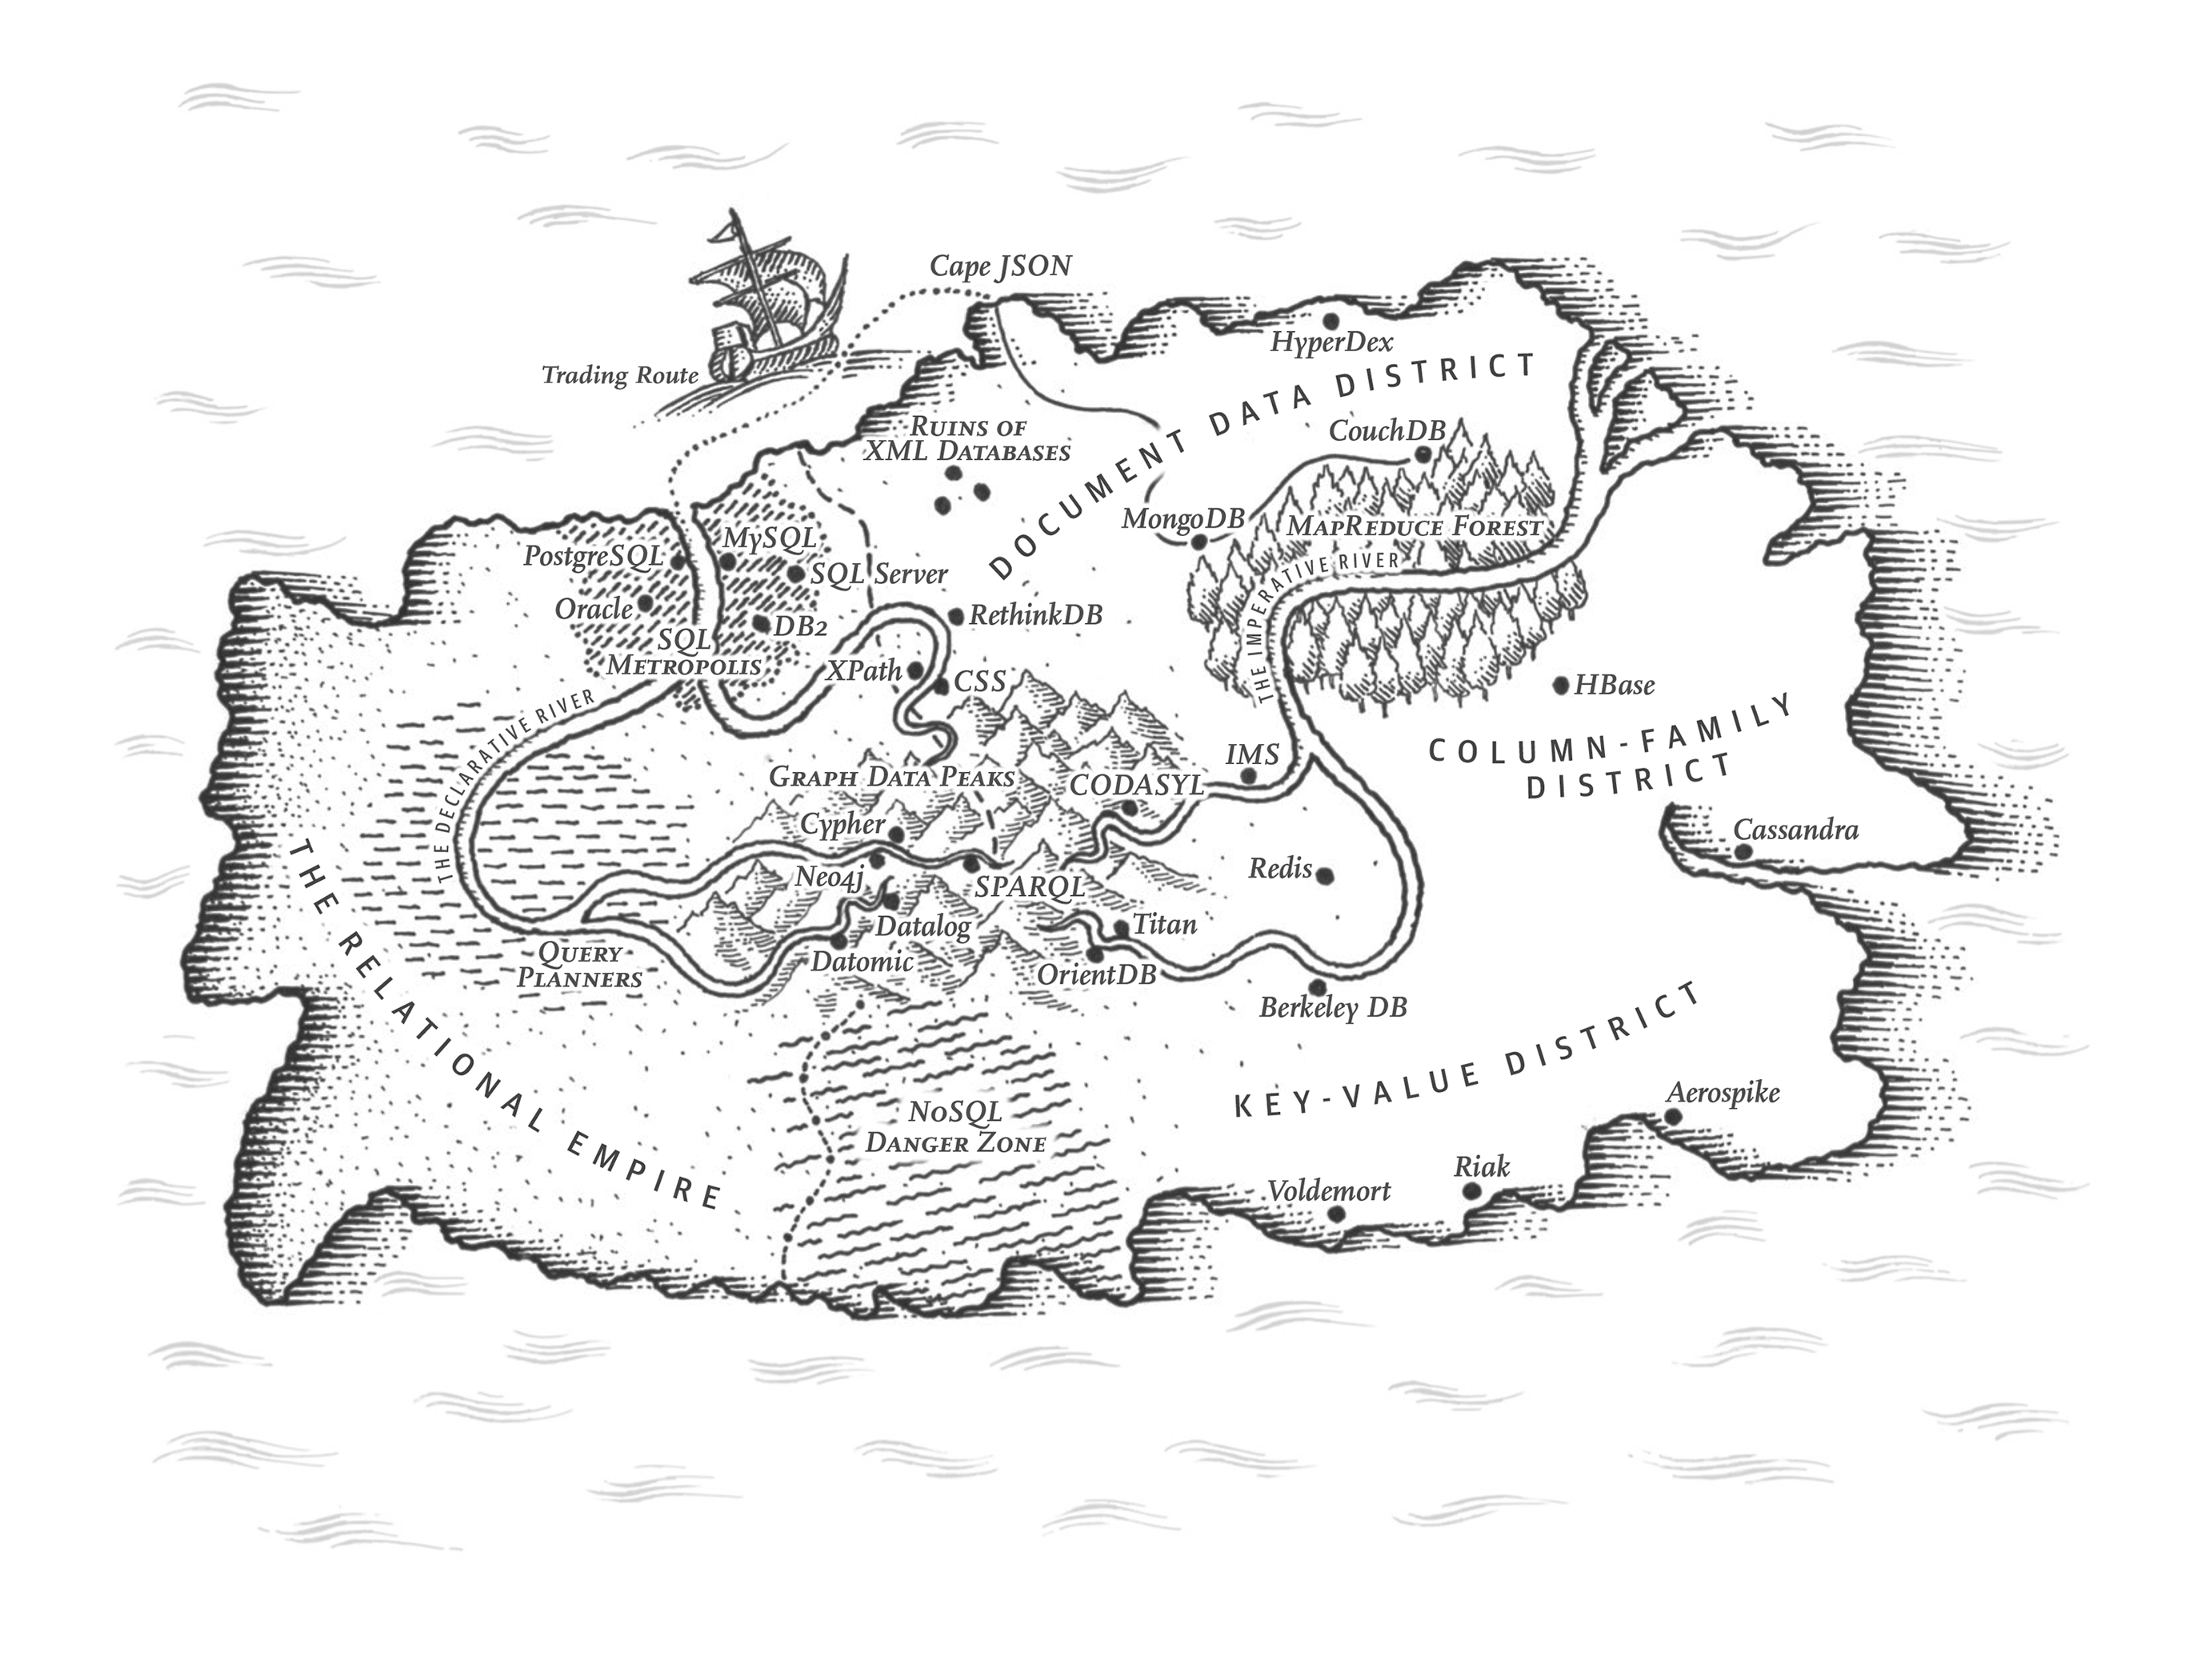
\includegraphics[width=\textwidth]{images/databases}
  }
\caption{A map of data storage techniques from Designing Data-Intensive Applications \cite{data-intensive}.}
\end{figure}

\section{This Week}
This week our goal is to:
\begin{itemize}
  \item explore the various techniques developers use to store data; and
  \item look at the storage options implementing these techniques on the AWS platform.
\end{itemize}

\section{Introduction}
Unfortunately, to build interesting software we often need to store and use data.
The storage of data introduces a number of challenges to designing, creating, and maintaining our software.
However, not all data storage techniques are created equal;
the choice of data storage model can have a profound impact on our software's complexity and maintainability.
In this practical, we want to take a superficial exploration our island of data storage models.
For a more in-depth treatment of data storage models that is outside the scope of this course,
see the \textit{Designing Data-Intensive Applications} book \cite{data-intensive}.

\section{Relational Storage}
\begin{itemize}
  \item Roll your own box.
  \item Amazon RDS.
  \item Amazon Aurora.
\end{itemize}

  \subsection{ORM}
  Just mentioning the relational-object mismatch.

  \subsection{Wide-Column Storage}
  \begin{itemize}
    \item Amazon Keyspaces (for Apache Cassandra)
  \end{itemize}

\section{Key-Value Storage}
\begin{itemize}
  \item Roll your own box.
  \item Amazon DynamoDB.
  \item Amazon ElastiCache.
  \item Amazon MemoryDB for Redis.
\end{itemize}

  \subsection{Time Series Storage}
  \begin{itemize}
    \item Amazon Timestream.
  \end{itemize}


\section{Document Storage}
\begin{itemize}
  \item Roll your own.
  \item Amazon DocumentDB.
\end{itemize}

\section{Graph Storage}
\begin{itemize}
  \item Amazon Neptune.
\end{itemize}



\bibliographystyle{ieeetr}
\bibliography{books}

\end{document}